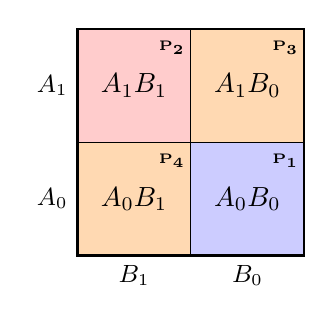
\begin{tikzpicture}[scale=1.2]
    % P2: A_1 B_1 (top-left)
    \draw[fill=red!20] (-1.8, 0.6) rectangle (-0.6, 1.8);
    \node at (-1.2, 1.2) {$A_1 B_1$};
    \node[font=\tiny, black] at (-0.8, 1.6) {$\mathbf{P_2}$};
    
    % P3: A_1 B_0 (top-right)
    \draw[fill=orange!30] (-0.6, 0.6) rectangle (0.6, 1.8);
    \node at (0, 1.2) {$A_1 B_0$};
    \node[font=\tiny, black] at (0.4, 1.6) {$\mathbf{P_3}$};
    
    % P4: A_0 B_1 (bottom-left)
    \draw[fill=orange!30] (-1.8, -0.6) rectangle (-0.6, 0.6);
    \node at (-1.2, 0) {$A_0 B_1$};
    \node[font=\tiny, black] at (-0.8, 0.4) {$\mathbf{P_4}$};
    
    % P1: A_0 B_0 (bottom-right)
    \draw[fill=blue!20] (-0.6, -0.6) rectangle (0.6, 0.6);
    \node at (0, 0) {$A_0 B_0$};
    \node[font=\tiny, black] at (0.4, 0.4) {$\mathbf{P_1}$};
    
    % Outer border
    \draw[thick] (-1.8, -0.6) rectangle (0.6, 1.8);
    
    % Labels for inputs
    % Vertical axis (A) - left side
    \node[left, font=\small] at (-1.8, 1.2) {$A_1$};
    \node[left, font=\small] at (-1.8, 0) {$A_0$};
    
    % Horizontal axis (B) - bottom
    \node[below, font=\small] at (-1.2, -0.6) {$B_1$};
    \node[below, font=\small] at (0, -0.6) {$B_0$};
\end{tikzpicture}
